\begin{figure}[tp]
	\centering
	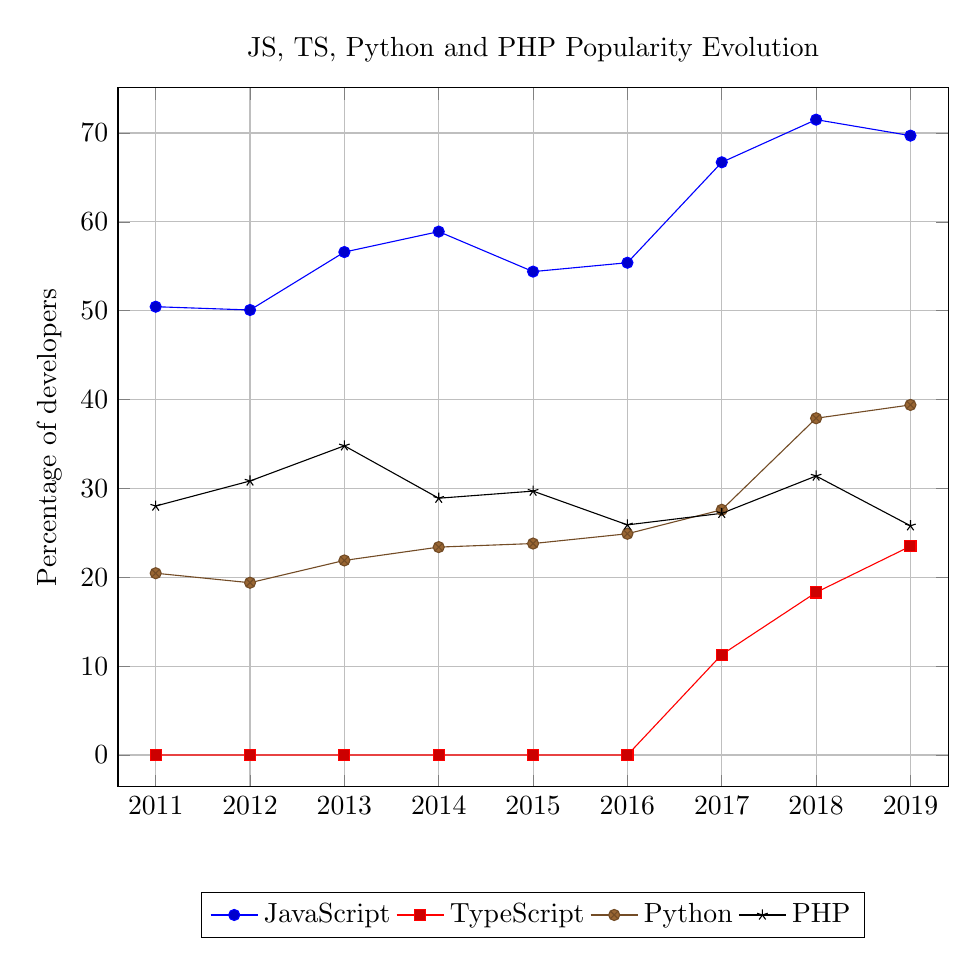
\begin{tikzpicture}
		\begin{axis}[
			width=1\textwidth,
			ylabel=Percentage of developers,
			title={JS, TS, Python and PHP Popularity Evolution},
			enlargelimits=0.05,
			legend style={at={(0.5,-0.15)},
				anchor=north,legend columns=-1},
			xticklabels={
				2011,
				2012,
				2013,
				2014,
				2015,
				2016,
				2017,
				2018,
				2019
			},
			xtick={0,...,8},
			grid=major,
		]

		% JavaScript
		\addplot coordinates {
			(0,50.45)
			(1,50.08)
			(2,56.60)
			(3,58.90)
			(4,54.40)
			(5,55.4)
			(6,66.7)
			(7,71.5)
			(8,69.7)
		};
		
		% TypeScript
		\addplot coordinates {
			(0,0)
			(1,0)
			(2,0)
			(3,0)
			(4,0)
			(5,0)
			(6,11.3)
			(7,18.3)
			(8,23.5)
		};
		
		% Python
		\addplot coordinates {
			(0,20.46)
			(1,19.39)
			(2,21.9)
			(3,23.4)
			(4,23.8)
			(5,24.9)
			(6,27.6)
			(7,37.9)
			(8,39.4)
		};

		% PHP
		\addplot coordinates {
			(0,28.02)
			(1,30.84)
			(2,34.8)
			(3,28.9)
			(4,29.7)
			(5,25.9)
			(6,27.2)
			(7,31.4)
			(8,25.8)
		};
		\legend{JavaScript,TypeScript,Python,PHP}
		\end{axis}
	\end{tikzpicture}
	\caption[Conditional operators]{\textbf{JS, TS, Python and PHP Popularity Evolution 2011 - 2019} - According to Stackoverflow's Developer Survey, for the seventh year in a row, JavaScript is the most commonly used programming language. While JavaScript's popularity remained constant for the last 3 years, TypeScript's popularity is increasing every year. There is no data for TypeScript before 2017.}
	\label{fig:background-programming-languages-evolution}
\end{figure}